\subsection{Algorytm Kruskala}

\textbf{Algorytm Kruskala} \cite{cormen2009} do znalezienia minimalnego drzewa rozpinającego wykorzystuje strukturę zbiorów rozłącznych (ang. \textit{Disjoint Set}).

Struktura \textit{Disjoint Set} reprezentuje rozłączne zbiory elementów za pomocą drzew. Na początku każdy element tworzy pojedynczy, jednoelementowy zbiór, którego reprezentantem jest korzeń drzewa. Główna operacja na tej strukturze, \textit{unia}, łączy dwa zbiory, tworząc jedno drzewo, w którym korzeń jednego zbioru staje się potomkiem korzenia drugiego. W ten sposób zbiory są scalane. Schematyczne przedstawienie scalania zbiorów znajduje się na Rysunku \ref{fig:disjoint_set}.

\begin{figure}[ht]
    \centering
    \begin{subfigure}{0.24\textwidth}
        \centering
        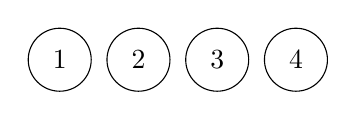
\begin{tikzpicture}[scale=1, every node/.style={circle,draw,minimum size=8mm}]
            \node (n0) at (0,0) {1};
            \node (n1) at (1,0) {2};
            \node (n3) at (2,0) {3};
            \node (n4) at (3,0) {4};
        \end{tikzpicture}
        \caption{Krok 1}
        \label{fig:disjoint_set_a}
    \end{subfigure}
    \begin{subfigure}{0.24\textwidth}
        \centering
        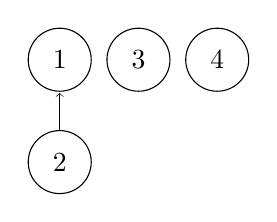
\begin{tikzpicture}[scale=1, every node/.style={circle,draw,minimum size=8mm}]
            \node (n0) at (0,1.3) {1};
            \node (n1) at (0,0) {2};
            \node (n2) at (1,1.3) {3};
            \node (n3) at (2,1.3) {4};
            \draw[->, very thin, black] (0,0.4) -- (0,0.88);
        \end{tikzpicture}
        \caption{Krok 2}
        \label{fig:disjoint_set_b}
    \end{subfigure}
    \begin{subfigure}{0.24\textwidth}
        \centering
        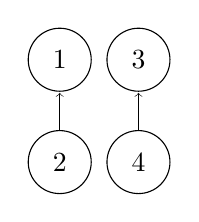
\begin{tikzpicture}[scale=1, every node/.style={circle,draw,minimum size=8mm}]
            \node (n0) at (0,1.3) {1};
            \node (n1) at (0,0) {2};
            \node (n2) at (1,1.3) {3};
            \node (n3) at (1,0) {4};
            \draw[->, very thin, black] (0,0.4) -- (0,0.88);
            \draw[->, very thin, black] (1,0.4) -- (1,0.88);
        \end{tikzpicture}
        \caption{Krok 3}
        \label{fig:disjoint_set_c}
    \end{subfigure}
    \hfill
    \begin{subfigure}{0.24\textwidth}
        \centering
        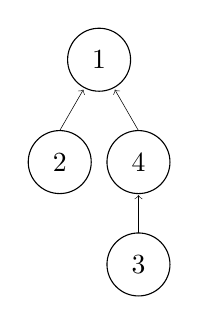
\begin{tikzpicture}[scale=1, every node/.style={circle,draw,minimum size=8mm}]
            \node (n0) at (0.5,2.6) {1};
            \node (n1) at (0,1.3) {2};
            \node (n2) at (1,0) {3};
            \node (n3) at (1,1.3) {4};
            \draw[->, very thin, black] (0,1.7) -- (0.3,2.22);
            \draw[->, very thin, black] (1,1.7) -- (0.7,2.22);
            \draw[->, very thin, black] (1,0.4) -- (1,0.88);
        \end{tikzpicture}
        \caption{Krok 4}
        \label{fig:disjoint_set_d}
    \end{subfigure}
    \caption{Kolejne kroki scalania zbioru}
    \label{fig:disjoint_set}
\end{figure}
%https://cp-algorithms.com/data_structures/disjoint_set_union.html

Projekt wykorzystuje zmodyfikowaną wersję algorytmu Kruskala. W klasycznym wariancie algorytm losowo wybiera krawędź, czyli parę sąsiadujących komórek, które mogą zostać połączone ścieżką. Jeśli komórki te należą do różnych zbiorów, są one łączone w jeden zbiór, a między nimi tworzone jest przejście.

W prezentowanej wersji algorytmu zamiast losowo wybierać krawędzie, iteruje się w losowej kolejności po wszystkich komórkach planszy. Dla każdej komórki rozpatrywani są jej sąsiedzi – jeśli należą do innych zbiorów, bieżąca komórka zostaje przekształcona w ścieżkę, a sąsiadujące zbiory zostają połączone.

Kluczową różnicą w porównaniu do klasycznego podejścia jest sposób zakończenia algorytmu. W tradycyjnej wersji wszystkie komórki zostają połączone w jeden wspólny zbiór. W tym przypadku natomiast, ze względu na lokalny charakter działania, istnieje wysokie prawdopodobieństwo, że w wyniku działania algorytmu pozostanie wiele niepołączonych zbiorów. Mimo to, końcowy układ labiryntu wizualnie przypomina ten uzyskany metodą klasyczną.

Poszczególne kroki generowania labiryntu przebiegają następująco:
\begin{enumerate}
    \item Tworzona jest siatka, w której wszystkie pola są początkowo oznaczone jako przejścia. Warto zaznaczyć, że nie ma znaczenia, czy algorytm rozpoczyna z planszą wypełnioną przejściami, a następnie tworzy ściany, czy odwrotnie — z planszą wypełnioną ścianami, w której tworzone są przejścia. Efekt końcowy pozostaje taki sam. Przykład planszy z samymi przejściami przedstawiono na \ref{fig:kruskal_step_1}.

    \begin{figure}[ht]
    \centering
    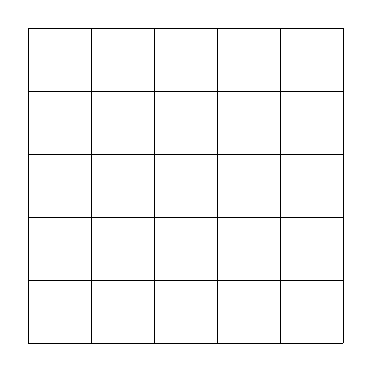
\begin{tikzpicture}[scale=0.8]
        \draw[step=1cm,ultra thin,black] (0,0) grid (5,5);
    \end{tikzpicture}
    \caption{\centering Cała plansza stanowi przejścia.}
    \label{fig:kruskal_step_1}
\end{figure}

    \item Każde pole planszy jest osobnym zbiorem w strukturze zbiorów rozłącznych. Na tym etapie żadna komórka nie jest jeszcze połączona z inną, co zostało przedstawione na Rysunku \ref{fig:kruskal_step_2}.

    \begin{figure}[H]
    \centering
    \begin{tikzpicture}[scale=0.8]
        \draw[step=1cm, ultra thin, black] (0,0) grid (5,5);
        
        \newcounter{char}
        \setcounter{char}{1}
        
        \foreach \x in {0,...,4} {
            \foreach \y in {0,...,4} {
                \ifnum\value{char}<26
                    \node at (\x + 0.5, 4.5 - \y) {\small\textbf{\Alph{char}}};
                    \stepcounter{char}
                \fi
            }
        }
    \end{tikzpicture}
    \caption{\centering Każdy zbiór jest oznaczony unikalną literą.}
    \label{fig:kruskal_step_2}
\end{figure}

    \item Komórki planszy są rozpatrywane w losowej kolejności:
    \begin{enumerate}
        \item Dla wybranej komórki określa się bezpośrednich sąsiadów. W tym przypadku są to pola bezpośrednio przyległe w górę, doł, lewo lub prawo - inaczej niż przyjęto w algorytmie Prima. Przykład takiej sytuacji przedstawiono na Rysunku \ref{fig:kruskal_step_3_a}.
        
        \begin{figure}[H]
    \centering
    \begin{tikzpicture}[scale=0.8]
        \draw[step=1cm, ultra thin, black] (0,0) grid (5,5);
        \draw (1.5,1.5) circle[radius=4mm];

        \fill[pattern=north east lines, pattern color=gray] (0,1) rectangle ++(1,1);
        \fill[pattern=north east lines, pattern color=gray] (1,0) rectangle ++(1,1);
        \fill[pattern=north east lines, pattern color=gray] (1,2) rectangle ++(1,1);
        \fill[pattern=north east lines, pattern color=gray] (2,1) rectangle ++(1,1);

        \newcounter{char_kruskal_3a}
        \setcounter{char_kruskal_3a}{1}
        \foreach \x in {0,...,4} {
            \foreach \y in {0,...,4} {
                \ifnum\value{char_kruskal_3a}<26
                    \node at (\x + 0.5, 4.5 - \y) {\small\textbf{\Alph{char_kruskal_3a}}};
                    \stepcounter{char_kruskal_3a}
                \fi
            }
        }
    \end{tikzpicture}
    \caption{\centering Losowa komórka (oznaczona kółkiem) i jej sąsiedzi (zakreskowani).}
    \label{fig:kruskal_step_3_a}
\end{figure}


        \item Jeśli wszyscy sąsiedzi należą do różnych zbiorów to wylosowana komórka staje się ścianą, a jej sąsiedzi są łączeni w jeden zbiór. Schemat łączenia komórek w zbiory pokazano na Rysunku \ref{fig:kruskal_step_3_b}.

        \begin{figure}[H]
    \centering
    \begin{tikzpicture}[scale=0.8]
        \draw[step=1cm, ultra thin, black] (0,0) grid (5,5);

        \newcounter{char_kruskal_3b}
        \setcounter{char_kruskal_3b}{1}
        \foreach \x in {0,...,4} {
            \foreach \y in {0,...,4} {
                \ifnum\value{char_kruskal_3b}<26
                    \node at (\x + 0.5, 4.5 - \y) {\small\textbf{\Alph{char_kruskal_3b}}};
                    \stepcounter{char_kruskal_3b}
                \fi
            }
        }

        \fill[white] (0.1,1.1) rectangle ++(0.8, 0.8);
        \fill[white] (1.1,0.1) rectangle ++(0.8, 0.8);
        \fill[white] (1.1,2.1) rectangle ++(0.8, 0.8);
        \fill[white] (2.1,1.1) rectangle ++(0.8, 0.8);

        \node at (0.5, 1.5) {\small\textbf{H}};
        \node at (1.5, 0.5) {\small\textbf{H}};
        \node at (1.5, 2.5) {\small\textbf{H}};
        \node at (2.5, 1.5) {\small\textbf{H}};

        \draw[ultra thick] (0, 1) -- (0, 2);
        \draw[ultra thick] (1, 0) -- (1, 1);
        \draw[ultra thick] (2, 0) -- (2, 1);
        \draw[ultra thick] (3, 1) -- (3, 2);
        \draw[ultra thick] (3, 1) -- (3, 2);
        \draw[ultra thick] (1, 2) -- (1, 3);
        \draw[ultra thick] (2, 2) -- (2, 3);

        \draw[ultra thick] (1, 0) -- (2, 0);
        \draw[ultra thick] (1, 3) -- (2, 3);
        \draw[ultra thick] (0, 2) -- (1, 2);
        \draw[ultra thick] (0, 1) -- (1, 1);
        \draw[ultra thick] (2, 1) -- (3, 1);
        \draw[ultra thick] (2, 2) -- (3, 2);

        \fill[gray] (1,1) rectangle ++(1,1);
    \end{tikzpicture}
    \caption{\centering Łączenie komórek w zbiory. Reprezentantem zbioru jest pierwszy dodany element (tutaj komórka H), choć może to być dowolna komórka z grupy.}
    \label{fig:kruskal_step_3_b}
\end{figure}


        \item Jeśli chociaż dwaj sąsiedzi należą do tego samego zbioru, komórka nie zostaje oznaczona jako ściana – pozostaje przejściem, co przedstawiono na Rysunku~\ref{fig:kruskal_step_3_c}.

        \begin{figure}[H]
    \centering
    \begin{subfigure}{0.45\textwidth}
        \centering
        \begin{tikzpicture}[scale=0.8]
            \draw[step=1cm, ultra thin, black] (0,0) grid (5,5);

            \newcounter{char_kruskal_3ca}
            \setcounter{char_kruskal_3ca}{1}
            \foreach \x in {0,...,4} {
                \foreach \y in {0,...,4} {
                    \ifnum\value{char_kruskal_3ca}<26
                        \node at (\x + 0.5, 4.5 - \y) {\small\textbf{\Alph{char_kruskal_3ca}}};
                        \stepcounter{char_kruskal_3ca}
                    \fi
                }
            }

            \fill[white] (0.1,1.1) rectangle ++(0.8, 0.8);
            \fill[white] (1.1,0.1) rectangle ++(0.8, 0.8);
            \fill[white] (1.1,2.1) rectangle ++(0.8, 0.8);
            \fill[white] (2.1,1.1) rectangle ++(0.8, 0.8);

            \fill[pattern=north east lines, pattern color=darkgray] (1,0) rectangle ++(1,1);
            \fill[pattern=north east lines, pattern color=darkgray] (2,1) rectangle ++(1,1);
            \fill[pattern=north east lines, pattern color=darkgray] (3,0) rectangle ++(1,1);

            \node at (0.5, 1.5) {\small\textbf{H}};
            \node at (1.5, 0.5) {\small\textbf{H}};
            \node at (1.5, 2.5) {\small\textbf{H}};
            \node at (2.5, 1.5) {\small\textbf{H}};

            \draw[ultra thick] (0, 1) -- (0, 2);
            \draw[ultra thick] (1, 0) -- (1, 1);
            \draw[ultra thick] (2, 0) -- (2, 1);
            \draw[ultra thick] (3, 1) -- (3, 2);
            \draw[ultra thick] (3, 1) -- (3, 2);
            \draw[ultra thick] (1, 2) -- (1, 3);
            \draw[ultra thick] (2, 2) -- (2, 3);

            \draw[ultra thick] (1, 0) -- (2, 0);
            \draw[ultra thick] (1, 3) -- (2, 3);
            \draw[ultra thick] (0, 2) -- (1, 2);
            \draw[ultra thick] (0, 1) -- (1, 1);
            \draw[ultra thick] (2, 1) -- (3, 1);
            \draw[ultra thick] (2, 2) -- (3, 2);

            \fill[gray] (1,1) rectangle ++(1,1);

            \draw (2.5,0.5) circle[radius=4mm];
        \end{tikzpicture}
        \caption{\centering Wylosowanie kolejnej komórki.}
        \label{fig:kruskal_step_3_c_a}
    \end{subfigure}
    \begin{subfigure}{0.45\textwidth}
        \centering
        \begin{tikzpicture}[scale=0.8]
            \draw[step=1cm, ultra thin, black] (0,0) grid (5,5);
            \newcounter{char_kruskal_3cb}
            \setcounter{char_kruskal_3cb}{1}
            \foreach \x in {0,...,4} {
                \foreach \y in {0,...,4} {
                    \ifnum\value{char_kruskal_3cb}<26
                        \node at (\x + 0.5, 4.5 - \y) {\small\textbf{\Alph{char_kruskal_3cb}}};
                        \stepcounter{char_kruskal_3cb}
                    \fi
                }
            }

            \fill[white] (0.1,1.1) rectangle ++(0.8, 0.8);
            \fill[white] (1.1,0.1) rectangle ++(0.8, 0.8);
            \fill[white] (1.1,2.1) rectangle ++(0.8, 0.8);
            \fill[white] (2.1,1.1) rectangle ++(0.8, 0.8);
            \fill[white] (2.1,0.1) rectangle ++(0.8, 0.8);

            \node at (0.5, 1.5) {\small\textbf{H}};
            \node at (1.5, 0.5) {\small\textbf{H}};
            \node at (1.5, 2.5) {\small\textbf{H}};
            \node at (2.5, 1.5) {\small\textbf{H}};

            \draw[ultra thick] (0, 1) -- (0, 2);
            \draw[ultra thick] (1, 0) -- (1, 1);
            \draw[ultra thick] (2, 0) -- (2, 1);
            \draw[ultra thick] (3, 1) -- (3, 2);
            \draw[ultra thick] (3, 1) -- (3, 2);
            \draw[ultra thick] (1, 2) -- (1, 3);
            \draw[ultra thick] (2, 2) -- (2, 3);

            \draw[ultra thick] (1, 0) -- (2, 0);
            \draw[ultra thick] (1, 3) -- (2, 3);
            \draw[ultra thick] (0, 2) -- (1, 2);
            \draw[ultra thick] (0, 1) -- (1, 1);
            \draw[ultra thick] (2, 1) -- (3, 1);
            \draw[ultra thick] (2, 2) -- (3, 2);

            \fill[gray] (1,1) rectangle ++(1,1);
        \end{tikzpicture}
        \caption{\centering Pozostawienie przejścia.}
        \label{fig:kruskal_step_3_c_b}
    \end{subfigure}
    \caption{\centering Wylosowana komórka ma już dwóch takich samych sąsiadów - scalanie nie następuje.}
    \label{fig:kruskal_step_3_c}
\end{figure}
    \end{enumerate}

    \item Proces powtarza się, aż każda komórka zostanie przetworzona. Przykładowe dalsze kroki algorytmu przedstawia Rysunek \ref{fig:kruskal_later_steps}, a Rysunek \ref{fig:kruskal_example_maze} ukazuje potencjalny schemat wygenerowanego labiryntu.
    
    \begin{figure}[H]
    \centering
    \begin{subfigure}{0.3\textwidth}
        \centering
        \begin{tikzpicture}[scale=0.8]
            \draw[step=1cm, ultra thin, black] (0,0) grid (5,5);

            \fill[lightlightgray] (2,0) rectangle ++(1, 1);
            \fill[lightlightgray] (2,2) rectangle ++(1, 1);

            \newcounter{char_kruskal_later_a}
            \setcounter{char_kruskal_later_a}{1}
            \foreach \x in {0,...,4} {
                \foreach \y in {0,...,4} {
                    \ifnum\value{char_kruskal_later_a}<26
                        \node at (\x + 0.5, 4.5 - \y) {\small\textbf{\Alph{char_kruskal_later_a}}};
                        \stepcounter{char_kruskal_later_a}
                    \fi
                }
            }

            \fill[white] (0.1,1.1) rectangle ++(0.8, 0.8);
            \fill[white] (1.1,0.1) rectangle ++(0.8, 0.8);
            \fill[white] (1.1,2.1) rectangle ++(0.8, 0.8);
            \fill[white] (2.1,1.1) rectangle ++(0.8, 0.8);

            \node at (0.5, 1.5) {\small\textbf{H}};
            \node at (1.5, 0.5) {\small\textbf{H}};
            \node at (1.5, 2.5) {\small\textbf{H}};
            \node at (2.5, 1.5) {\small\textbf{H}};

            \draw[ultra thick] (0, 1) -- (0, 2);
            \draw[ultra thick] (1, 0) -- (1, 1);
            \draw[ultra thick] (2, 0) -- (2, 1);
            \draw[ultra thick] (3, 1) -- (3, 2);
            \draw[ultra thick] (3, 1) -- (3, 2);
            \draw[ultra thick] (1, 2) -- (1, 3);
            \draw[ultra thick] (2, 2) -- (2, 3);

            \draw[ultra thick] (1, 0) -- (2, 0);
            \draw[ultra thick] (1, 3) -- (2, 3);
            \draw[ultra thick] (0, 2) -- (1, 2);
            \draw[ultra thick] (0, 1) -- (1, 1);
            \draw[ultra thick] (2, 1) -- (3, 1);
            \draw[ultra thick] (2, 2) -- (3, 2);

            \fill[gray] (1,1) rectangle ++(1,1);
        \end{tikzpicture}
        \caption{\centering Kolejna komórka bez unikalnych sąsiadów.}
        \label{fig:kruskal_later_steps_a}
    \end{subfigure}
    \begin{subfigure}{0.3\textwidth}
        \centering
        \begin{tikzpicture}[scale=0.8]
            \draw[step=1cm, ultra thin, black] (0,0) grid (5,5);

            \fill[lightlightgray] (2,0) rectangle ++(1, 1);
            \fill[lightlightgray] (2,2) rectangle ++(1, 1);

            \fill[gray] (1,1) rectangle ++(1,1);
            \fill[gray] (0,1) rectangle ++(1,1);

            \newcounter{char_kruskal_later_b}
            \setcounter{char_kruskal_later_b}{1}
            \foreach \x in {0,...,4} {
                \foreach \y in {0,...,4} {
                    \ifnum\value{char_kruskal_later_b}<26
                        \node at (\x + 0.5, 4.5 - \y) {\small\textbf{\Alph{char_kruskal_later_b}}};
                        \stepcounter{char_kruskal_later_b}
                    \fi
                }
            }

            \fill[gray] (0.1,1.1) rectangle ++(0.8, 0.8);

            \fill[white] (1.1,0.1) rectangle ++(0.8, 0.8);
            \fill[white] (1.1,2.1) rectangle ++(0.8, 0.8);
            \fill[white] (2.1,1.1) rectangle ++(0.8, 0.8);
            \fill[white] (0.1,2.1) rectangle ++(0.8, 0.8);
            \fill[white] (0.1,0.1) rectangle ++(0.8, 0.8);

            \node at (0.5, 1.5) {\small\textbf{H}};
            \node at (1.5, 0.5) {\small\textbf{H}};
            \node at (1.5, 2.5) {\small\textbf{H}};
            \node at (2.5, 1.5) {\small\textbf{H}};
            \node at (0.5, 0.5) {\small\textbf{H}};
            \node at (0.5, 2.5) {\small\textbf{H}};

            \draw[ultra thick] (0, 1) -- (0, 2);
            \draw[ultra thick] (2, 0) -- (2, 1);
            \draw[ultra thick] (3, 1) -- (3, 2);
            \draw[ultra thick] (2, 2) -- (2, 3);

            \draw[ultra thick] (1, 0) -- (2, 0);
            \draw[ultra thick] (1, 3) -- (2, 3);
            \draw[ultra thick] (2, 1) -- (3, 1);
            \draw[ultra thick] (2, 2) -- (3, 2);
            \draw[ultra thick] (0, 0) -- (0, 1);
            \draw[ultra thick] (0, 0) -- (1, 0);
            \draw[ultra thick] (0, 2) -- (0, 3);
            \draw[ultra thick] (0, 3) -- (1, 3);

        \end{tikzpicture}
        \caption{\centering Rozszerzenie połączonego zbioru.}
        \label{fig:kruskal_later_steps_b}
    \end{subfigure}
    \begin{subfigure}{0.3\textwidth}
        \centering
        \begin{tikzpicture}[scale=0.8]
            \draw[step=1cm, ultra thin, black] (0,0) grid (5,5);

            \fill[lightlightgray] (2,0) rectangle ++(1, 1);
            \fill[lightlightgray] (2,2) rectangle ++(1, 1);

            \fill[gray] (1,1) rectangle ++(1,1);
            \fill[gray] (0,1) rectangle ++(1,1);
            \fill[gray] (3,3) rectangle ++(1,1);

            \newcounter{char_kruskal_later_c}
            \setcounter{char_kruskal_later_c}{1}
            \foreach \x in {0,...,4} {
                \foreach \y in {0,...,4} {
                    \ifnum\value{char_kruskal_later_c}<26
                        \node at (\x + 0.5, 4.5 - \y) {\small\textbf{\Alph{char_kruskal_later_c}}};
                        \stepcounter{char_kruskal_later_c}
                    \fi
                }
            }

            \fill[gray] (0.1,1.1) rectangle ++(0.8, 0.8);

            \fill[white] (1.1,0.1) rectangle ++(0.8, 0.8);
            \fill[white] (1.1,2.1) rectangle ++(0.8, 0.8);
            \fill[white] (2.1,1.1) rectangle ++(0.8, 0.8);
            \fill[white] (0.1,2.1) rectangle ++(0.8, 0.8);
            \fill[white] (0.1,0.1) rectangle ++(0.8, 0.8);
            \fill[white] (2.1,3.1) rectangle ++(0.8, 0.8);
            \fill[white] (3.1,2.1) rectangle ++(0.8, 0.8);
            \fill[white] (3.1,4.1) rectangle ++(0.8, 0.8);
            \fill[white] (4.1,3.1) rectangle ++(0.8, 0.8);

            \node at (0.5, 1.5) {\small\textbf{H}};
            \node at (1.5, 0.5) {\small\textbf{H}};
            \node at (1.5, 2.5) {\small\textbf{H}};
            \node at (2.5, 1.5) {\small\textbf{H}};
            \node at (0.5, 0.5) {\small\textbf{H}};
            \node at (0.5, 2.5) {\small\textbf{H}};

            \node at (2.5, 3.5) {\small\textbf{P}};
            \node at (4.5, 3.5) {\small\textbf{P}};
            \node at (3.5, 2.5) {\small\textbf{P}};
            \node at (3.5, 4.5) {\small\textbf{P}};

            \draw[ultra thick] (0, 1) -- (0, 2);
            \draw[ultra thick] (2, 0) -- (2, 1);
            \draw[ultra thick] (3, 1) -- (3, 2);
            \draw[ultra thick] (2, 2) -- (2, 3);

            \draw[ultra thick] (1, 0) -- (2, 0);
            \draw[ultra thick] (1, 3) -- (2, 3);
            \draw[ultra thick] (2, 1) -- (3, 1);
            \draw[ultra thick] (2, 2) -- (3, 2);
            \draw[ultra thick] (0, 0) -- (0, 1);
            \draw[ultra thick] (0, 0) -- (1, 0);
            \draw[ultra thick] (0, 2) -- (0, 3);
            \draw[ultra thick] (0, 3) -- (1, 3);

            \draw[densely dashed, ultra thick] (2, 3) -- (3, 3);
            \draw[densely dashed, ultra thick] (4, 3) -- (5, 3);
            \draw[densely dashed, ultra thick] (2, 4) -- (3, 4);
            \draw[densely dashed, ultra thick] (4, 4) -- (5, 4);
            \draw[densely dashed, ultra thick] (3, 5) -- (4, 5);
            \draw[densely dashed, ultra thick] (3, 2) -- (4, 2);
            
            \draw[densely dashed, ultra thick] (2, 3) -- (2, 4);
            \draw[densely dashed, ultra thick] (5, 3) -- (5, 4);
            \draw[densely dashed, ultra thick] (3, 4) -- (3, 5);
            \draw[densely dashed, ultra thick] (3, 2) -- (3, 3);
            \draw[densely dashed, ultra thick] (4, 2) -- (4, 3);
            \draw[densely dashed, ultra thick] (4, 4) -- (4, 5);

        \end{tikzpicture}
        \caption{\centering Scalenie kolejnego zbioru.}
        \label{fig:kruskal_later_steps_c}
    \end{subfigure}
    \caption{Przykładowe kolejne iteracje algorytmu.}
    \label{fig:kruskal_later_steps}
\end{figure}

    \begin{figure}[ht]
    \centering
    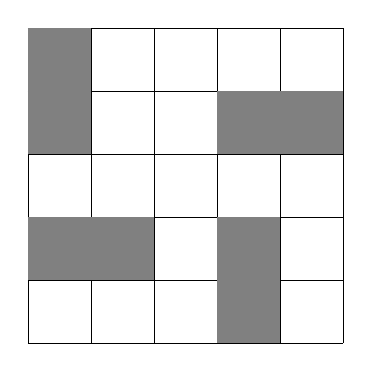
\begin{tikzpicture}[scale=0.8]
        \draw[step=1cm,ultra thin,black] (0,0) grid (5,5);

        \fill[gray] (1,1) rectangle ++(1,1);
        \fill[gray] (0,1) rectangle ++(1,1);
        \fill[gray] (3,3) rectangle ++(1,1);
        \fill[gray] (4,3) rectangle ++(1,1);
        \fill[gray] (0,3) rectangle ++(1,1);
        \fill[gray] (0,4) rectangle ++(1,1);
        \fill[gray] (0,4) rectangle ++(1,1);
        \fill[gray] (3,0) rectangle ++(1,1);
        \fill[gray] (3,1) rectangle ++(1,1);
    \end{tikzpicture}
    \caption{\centering Przykładowy wygląd końcowego, wygenerowanego labiryntu.}
    \label{fig:kruskal_example_maze}
\end{figure}
\end{enumerate}

\clearpage